\documentclass[tikz,border=4pt]{standalone}
\usepackage{amsmath,amssymb}
\usetikzlibrary{positioning,arrows.meta,calc,fit,backgrounds,shapes.misc}
\definecolor{new}{HTML}{2A78D6}
\definecolor{newbg}{HTML}{E4EFFB}
\definecolor{adapt}{HTML}{1BAF7A}
\definecolor{adaptbg}{HTML}{E2F5EE}
\definecolor{exist}{HTML}{6B6A64}
\definecolor{existbg}{HTML}{F0EFEC}
\definecolor{cal}{HTML}{EB6834}
\definecolor{calbg}{HTML}{FCEBE3}
\definecolor{ink}{HTML}{1A1A19}
\begin{document}
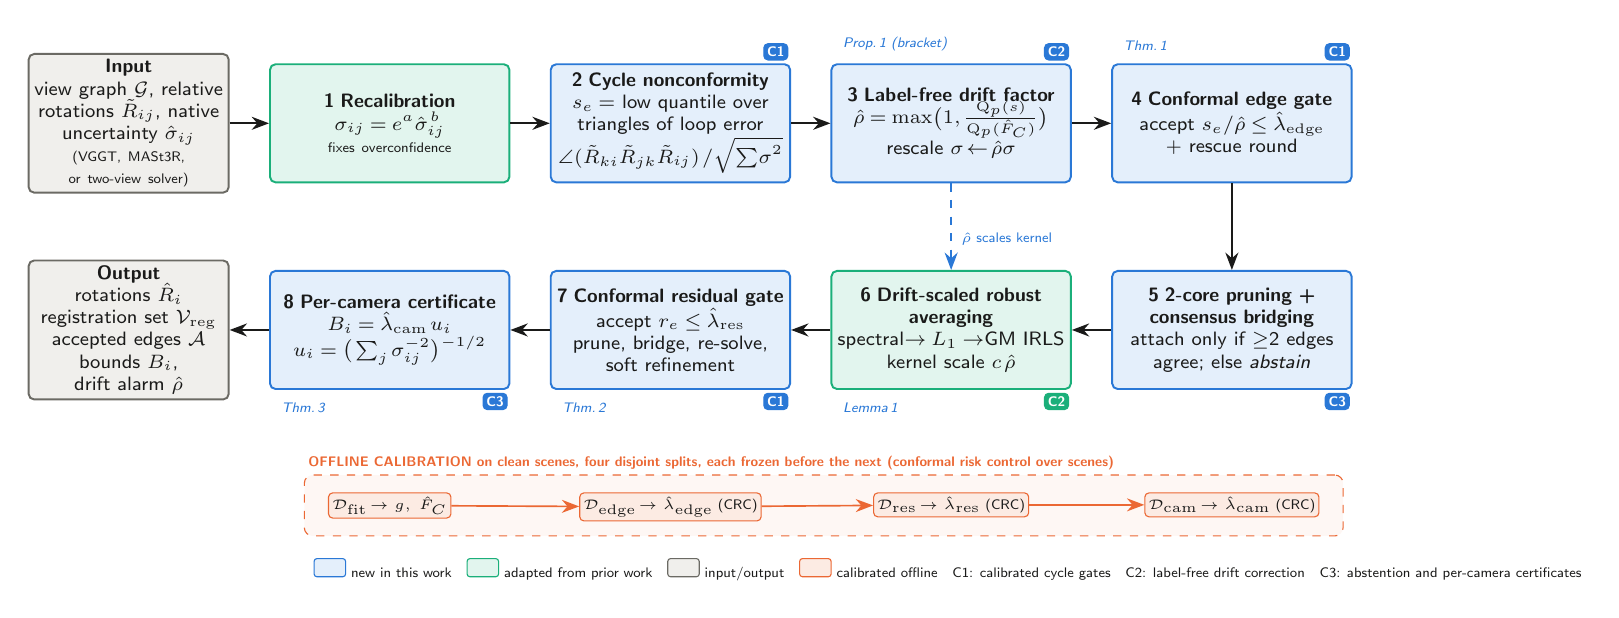
\begin{tikzpicture}[
  font=\sffamily\scriptsize, >={Stealth[length=2.2mm]}, ink,
  blk/.style={execute at begin node={\thickmuskip=4mu\medmuskip=3mu\thinmuskip=2mu}, draw, rounded corners=2pt, line width=0.7pt, align=center, text width=29mm, minimum height=15mm, inner sep=2pt},
  newb/.style={blk, draw=new, fill=newbg},
  adb/.style={blk, draw=adapt, fill=adaptbg},
  exb/.style={blk, draw=exist, fill=existbg},
  tag/.style={draw=new, fill=new, text=white, rounded corners=1.5pt, inner sep=1.2pt, font=\sffamily\bfseries\tiny},
  tagA/.style={draw=adapt, fill=adapt, text=white, rounded corners=1.5pt, inner sep=1.2pt, font=\sffamily\bfseries\tiny},
  chip/.style={draw=cal, fill=calbg, text=ink, rounded corners=1.5pt, inner sep=1.3pt, font=\sffamily\tiny},
  thm/.style={text=new, font=\sffamily\itshape\tiny},
  flow/.style={->, line width=0.8pt, draw=ink},
]
% ---------------- row 1 (left to right)
\node[exb, text width=24mm] (in) at (0,0) {\textbf{Input}\\view graph $\mathcal{G}$, relative\\rotations $\tilde R_{ij}$, native\\uncertainty $\hat\sigma_{ij}$\\{\tiny(VGGT, MASt3R,}\\{\tiny or two-view solver)}};
\node[adb, right=5mm of in] (b1) {\textbf{1\;Recalibration}\\$\sigma_{ij}=e^{a}\hat\sigma_{ij}^{\,b}$\\{\tiny fixes overconfidence}};
\node[newb, right=5mm of b1] (b2) {\textbf{2\;Cycle nonconformity}\\$s_e=$ low quantile over\\triangles of loop error\\$\angle(\tilde R_{ki}\tilde R_{jk}\tilde R_{ij})\,/\sqrt{\textstyle\sum\!\sigma^2}$};
\node[newb, right=5mm of b2] (b3) {\textbf{3\;Label-free drift factor}\\$\hat\rho=\max\!\big(1,\frac{\mathrm{Q}_p(s)}{\mathrm{Q}_p(\hat F_C)}\big)$\\rescale $\sigma\!\leftarrow\!\hat\rho\sigma$};
\node[newb, right=5mm of b3] (b4) {\textbf{4\;Conformal edge gate}\\accept $s_e/\hat\rho\le\hat\lambda_{\mathrm{edge}}$\\+ rescue round};
% ---------------- row 2 (right to left)
\node[newb, below=11mm of b4] (b5) {\textbf{5\;2-core pruning +}\\\textbf{consensus bridging}\\attach only if $\ge$2 edges\\agree; else \emph{abstain}};
\node[adb, left=5mm of b5] (b6) {\textbf{6\;Drift-scaled robust}\\\textbf{averaging}\\spectral$\to L_1\to$GM IRLS\\kernel scale $c\,\hat\rho$};
\node[newb, left=5mm of b6] (b7) {\textbf{7\;Conformal residual gate}\\accept $r_e\le\hat\lambda_{\mathrm{res}}$\\prune, bridge, re-solve,\\soft refinement};
\node[newb, left=5mm of b7] (b8) {\textbf{8\;Per-camera certificate}\\$B_i=\hat\lambda_{\mathrm{cam}}\,u_i$\\$u_i=\big(\sum_j\sigma_{ij}^{-2}\big)^{-1/2}$};
\node[exb, text width=24mm, left=5mm of b8] (out) {\textbf{Output}\\rotations $\hat R_i$\\registration set $\mathcal{V}_{\mathrm{reg}}$\\accepted edges $\mathcal{A}$\\bounds $B_i$, drift alarm $\hat\rho$};
% ---------------- flow
\draw[flow] (in) -- (b1); \draw[flow] (b1) -- (b2); \draw[flow] (b2) -- (b3); \draw[flow] (b3) -- (b4);
\draw[flow] (b4) -- (b5); \draw[flow] (b5) -- (b6); \draw[flow] (b6) -- (b7); \draw[flow] (b7) -- (b8); \draw[flow] (b8) -- (out);
\draw[flow, dashed, draw=new] (b3.south) -- ++(0,-3.2mm) -| node[pos=0.75, right, text=new, font=\sffamily\tiny]{$\hat\rho$ scales kernel} (b6.north);
% ---------------- contribution tags
\node[tag, anchor=south east] at ($(b2.north east)+(-1pt,1pt)$) {C1};
\node[tag, anchor=south east] at ($(b3.north east)+(-1pt,1pt)$) {C2};
\node[tag, anchor=south east] at ($(b4.north east)+(-1pt,1pt)$) {C1};
\node[tag, anchor=north east] at ($(b5.south east)+(-1pt,-1pt)$) {C3};
\node[tagA, anchor=north east] at ($(b6.south east)+(-1pt,-1pt)$) {C2};
\node[tag, anchor=north east] at ($(b7.south east)+(-1pt,-1pt)$) {C1};
\node[tag, anchor=north east] at ($(b8.south east)+(-1pt,-1pt)$) {C3};
% ---------------- guarantee labels
\node[thm, anchor=south west] at ($(b3.north west)+(1pt,1pt)$) {Prop.\,1 (bracket)};
\node[thm, anchor=south west] at ($(b4.north west)+(1pt,1pt)$) {Thm.\,1};
\node[thm, anchor=north west] at ($(b6.south west)+(1pt,-1pt)$) {Lemma\,1};
\node[thm, anchor=north west] at ($(b7.south west)+(1pt,-1pt)$) {Thm.\,2};
\node[thm, anchor=north west] at ($(b8.south west)+(1pt,-1pt)$) {Thm.\,3};
% ---------------- calibration lane
\coordinate (cy) at ($(b8.south)+(0,-13mm)$);
\node[chip, anchor=north] (c1) at (b1.south |- cy) {$\mathcal{D}_{\mathrm{fit}}\!\to g,\ \hat F_C$};
\node[chip, anchor=north] (c2) at (b7.south |- cy) {$\mathcal{D}_{\mathrm{edge}}\!\to\hat\lambda_{\mathrm{edge}}$ (CRC)};
\node[chip, anchor=north] (c3) at (b6.south |- cy) {$\mathcal{D}_{\mathrm{res}}\!\to\hat\lambda_{\mathrm{res}}$ (CRC)};
\node[chip, anchor=north] (c4) at (b5.south |- cy) {$\mathcal{D}_{\mathrm{cam}}\!\to\hat\lambda_{\mathrm{cam}}$ (CRC)};
\draw[->, cal, line width=0.6pt] (c1) -- (c2); \draw[->, cal, line width=0.6pt] (c2) -- (c3); \draw[->, cal, line width=0.6pt] (c3) -- (c4);
\begin{scope}[on background layer]
\node[draw=cal, fill=calbg!40, rounded corners=3pt, dashed, fit=(c1)(c4), inner xsep=3mm, inner ysep=2.2mm, label={[anchor=south west, text=cal, font=\sffamily\bfseries\tiny, inner sep=1.5pt]north west:OFFLINE CALIBRATION on clean scenes, four disjoint splits, each frozen before the next (conformal risk control over scenes)}] (calbox) {};
\end{scope}
% ---------------- legend
\node[anchor=north west, font=\sffamily\tiny, align=left] at ($(calbox.south west)+(0,-1.5mm)$) {%
\tikz\node[draw=new, fill=newbg, minimum width=4mm, minimum height=2.3mm, rounded corners=1pt]{}; new in this work\quad
\tikz\node[draw=adapt, fill=adaptbg, minimum width=4mm, minimum height=2.3mm, rounded corners=1pt]{}; adapted from prior work\quad
\tikz\node[draw=exist, fill=existbg, minimum width=4mm, minimum height=2.3mm, rounded corners=1pt]{}; input/output\quad
\tikz\node[draw=cal, fill=calbg, minimum width=4mm, minimum height=2.3mm, rounded corners=1pt]{}; calibrated offline\quad
C1: calibrated cycle gates\quad C2: label-free drift correction\quad C3: abstention and per-camera certificates};
\end{tikzpicture}
\end{document}
